\documentclass[11pt,a4paper]{article}

\usepackage{geometry}
\usepackage[spanish, activeacute]{babel}
\usepackage[utf8]{inputenc}
\usepackage{amsthm}
\usepackage{amsmath}
\usepackage{xfrac}
\usepackage{amsfonts}
\usepackage{amssymb}
\usepackage{graphicx}		% \includegraphics
\usepackage{float}			% Para fijar figuras y tablas exactamente donde uno quiere.
\usepackage{color}
\usepackage{clrscode3e}		% Algoritmos tipo CLRS.
\usepackage{caratula} 		% Utilitarios para armar la caratula.
\usepackage{euler}			% Texto matematico estilo Concrete Mathematics
\usepackage{url}            % Para hacer hipervínculos

\usepackage{footnote}
\makesavenoteenv{tabular}	% Para poner la footnote del capo del sorting.

\setcounter{secnumdepth}{5}

\renewcommand{\rmdefault}{pplx}	% Fuente estilo Concrete Mathematics.

% Codigo fuente.
\usepackage{listings}
\lstset{
	language=C++,
	basicstyle=\small\sffamily,
	numbers=left,
	numberstyle=\tiny,
	frame=tb,
	columns=fullflexible,
	showstringspaces=false
}

\newcommand\todo[1]{\Large\textbf{\textcolor{red}{#1}}\normalsize}


\usepackage{chngcntr}	% Numeracion granular de distintos entornos.
\counterwithin{table}{section}
\AtBeginDocument{\counterwithin{lstlisting}{section}}


\newtheorem{teo}{\textbf{Teorema}}[section]
\newtheorem{prop}{\textbf{Proposición}}[section]
\newtheorem{coro}{\textbf{Corolario}}[section]
\newtheorem{lema}{\textbf{Lema}}[section]
\newtheorem{afir}{\textbf{Afirmación}}[section]
\newtheorem{obs}{\textbf{Observación}}[section]
\theoremstyle{definition}
\newtheorem{defi}{\textbf{Definición}}[section]


% Tablas de archivos de test.
\usepackage{verbatim}	% \verbatiminput
\newcommand{\inoutsamplesfile}[3]{
     %\vspace{1\baselineskip}
     \begin{table}[H]
     %\newcommand{\testdir}{tests}
     \renewcommand{\tablename}{Test}
     \caption{\texttt{#3}}
     \begin{center}
     \begin{tabular}{|l|l|} \hline
          \textbf{Entrada} & \textbf{Salida} \\ \hline
          \begin{minipage}[t]{0.45\textwidth} \verbatiminput{#1} \vspace{-2ex} \end{minipage} & \begin{minipage}[t]{0.45\textwidth} \verbatiminput{#2} \vspace{-2ex} \end{minipage} \\ \hline
     \end{tabular}
     \end{center}
     \end{table}
}


\begin{document}

\parskip=5pt

\thispagestyle{empty}

% Caratula.
\def\Materia{Metaheurísticas}
\def\Titulo{Trabajo Pr'actico}
\def\Fecha{2 de septiembre de 2016}

\begin{center}
    {\LARGE\textbf{\Materia}}\\[1em]    
    \vspace{5mm}
    {\Large \textbf{\Titulo}}\\[1em]
    \vspace{2mm}
    {\textbf{\large \Fecha}}\\
    \vspace{5mm}
    \textbf{\tablaints}
\end{center}

\tableofcontents

\newpage

\pagestyle{headings}
\setcounter{page}{1}

%\input{ejemplos}
\newpage
\section{Introduccion Teorica}\label{sec:introduccion}
\subsection{Colonia de Hormigas}
Es una metaheuristica de la familia de PSO (Particle Swarm Optimization) basada en el comportamiento en grupo de las hormigas para definir el camino a un recurso deseado, en otras palabras es una metodología inspirada en el comportamiento colectivo de las hormigas en su búsqueda de alimentos. 
Es muy usada para solucionar problemas computacionales que pueden reducirse a buscar los mejores caminos o rutas en grafos es por eso que es muy importante recordar que las hormigas son prácticamente ciegas, y sin embargo, moviéndose prácticamente al azar, acaban encontrando el camino más corto desde su nido hasta la fuente de alimentos (y regresar).
Entre sus principales caracteristicas se encuentran:

\begin{enumerate}
\item Una sola hormiga no es capaz de realizar todo el trabajo sino que termina siendo el resultado de muchas hormigas en conjunto.
\item Una hormiga, cuando se mueve, deja una señal química en el suelo, depositando una sustancia denominada \textbf{feromona}, para que las demás puedan seguirla.
\end{enumerate}

De esta forma, aunque una hormiga aislada se mueva esencialmente al azar, las siguientes decidirán sus movimientos considerando seguir con mayor frecuencia el camino con mayor cantidad de feromonas.

La metaheuristica general consiste de lo siguiente:
\begin{enumerate}
\item En principio, todas las hormigas se mueven de manera aleatoria, buscando por si solas un camino al recurso que estan buscando (una posible solucion).
\item Una vez encontrada una solucion, la hormiga vuelve dejando un rastro de feromonas; este rastro puede ser mayor o menor dependiendo de lo buena que sea la solucion encontrada. 
\item Utilizando este rastro de feromonas, las hormigas pueden compartir informacion entre sus distintos pares en la colonia.
\item Cuando una nueva hormiga inicia su trabajo, es influenciada por la feromona depositada por las hormigas anteriores, y asi aumenta las probabilidades de que esta siga los pasos de sus anteriores
al acercarse a un recurso previamente encontrado.
\end{enumerate}


\begin{figure}[h]
\centering
\caption{Ejemplo convergencia a una solucion}
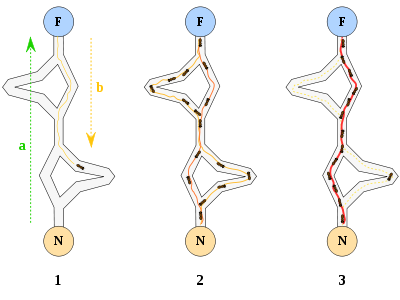
\includegraphics[width=5cm]{imagenes/feromona}
\end{figure}

\begin{figure}[h]
\caption{Ejemplo de uso de feromona}
\centering
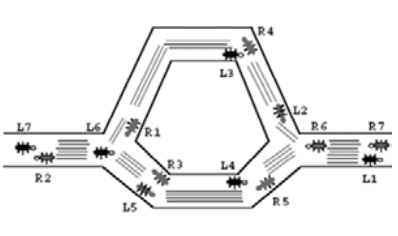
\includegraphics[width=5cm]{imagenes/feromona2}
\end{figure}

En la \textbf{figura 1} podemos ver una serie de iteraciones donde las hormigas llegan a la Fuente de comida y vuelven dejando feromonas y en la siguiente iteracion la solucion se ve influenciada por la feromona. Finalmente se lleva a una camino, el cual es elegido por casi todas las hormigas, siendo este la solucion final.

En la \textbf{figura 2} asumiendo que el nomero de lineas punteadas es proporcional a la cantidad de feromona, se puede ver como el camino inferior es más corto que el superior, muchas más hormigas transitarán por éste durante el mismo periodo de tiempo. Esto implica que en el camino más corto se acumula más feromona mucho más rápido. Después de cierto tiempo, la diferencia en la cantidad de feromona en los dos caminos es lo suficientemente grande para influenciar la decisión de las nuevas hormigas que entren a recorrer estas vías

Se puede ver que una gran ventaja de esta metaheuristica es que puede construir una solucion intercambiando informacion entre las distintas hormgias (soluciones), asi generar una solucion mejor de la que podrian generar individualmente.

Con el paso del tiempo el rastro de feromonas comienza a evaporarse, esto produce que los caminos pierdan su fuerza de atraccion, cuanto mas largo sea el camino, mas tiempo demorara una hormiga en recorrerlo, mas se evaporara la feromona y por ende seran menos frecuentado. Por su parte los caminos mas cortos (o mas optimos) tendran mayor cantidad de feromonas, por ende, mayor probabilidad de ser frecuentados.

ACO fue el primer algoritmo de optimizacion de Colonias de Hormigas desarrollado por Marco Dorigo en su tesis doctoral \cite{paperDorigo}. 

Algunas de las aplicaciones donde se utiliza esta metaheuristica:
\begin{enumerate}
\item El problema del viajante de comercion (TSP)
\item Optimización para el diseño de circuitos lógicos combinatorios
\item Problemas de enrutamiento de vehículos
\item Problema de la asignación de horarios
\item Aplicaciones a análisis de ADN y a procesos de producción
\item Partición de un grafo en árboles:
\item Otros
\end{enumerate}



\begin{thebibliography}{9}
\bibitem{wikipedia} 
https://en.wikipedia.org/wiki/Ant\_colony\_optimization\_algorithms

\bibitem{claseMetah} 
http://www-2.dc.uba.ar/materias/metah/meta2016-clase7.pdf

 
\bibitem{paperDorigo} 
http://people.idsia.ch/~gianni/Papers/CEC99.pdf

\bibitem{paperAplicaciones} 
Ant colony optimization: applications and trends. Carlos Algarin

\end{thebibliography}
\newpage
\section{El problema}\label{sec:problema}

Lorem ipsum dolor sit amet, consectetur adipisicing elit, sed do eiusmod
tempor incididunt ut labore et dolore magna aliqua. Ut enim ad minim veniam,
quis nostrud exercitation ullamco laboris nisi ut aliquip ex ea commodo
consequat. Duis aute irure dolor in reprehenderit in voluptate velit esse
cillum dolore eu fugiat nulla pariatur. Excepteur sint occaecat cupidatat non
proident, sunt in culpa qui officia deserunt mollit anim id est laborum.
\newpage
\section{Algoritmo Propuesto}\label{sec:algoritmo}
\subsection{Explicacion}

Lorem ipsum dolor sit amet, consectetur adipisicing elit, sed do eiusmod
tempor incididunt ut labore et dolore magna aliqua. Ut enim ad minim veniam,
quis nostrud exercitation ullamco laboris nisi ut aliquip ex ea commodo
consequat. Duis aute irure dolor in reprehenderit in voluptate velit esse
cillum dolore eu fugiat nulla pariatur. Excepteur sint occaecat cupidatat non
proident, sunt in culpa qui officia deserunt mollit anim id est laborum.

\subsection{Pseudocodigo}

\begin{codebox}
\Procname{$\proc{Insertion-Sort}(A)$}
\li \For $j \gets 2$ \To $\attrib{A}{length}$
\li \Do
$\id{key} \gets A[j]$
\li \Comment Insert $A[j]$ into the sorted sequence
$A[1 \twodots j-1]$.
\li $i \gets j-1$
\li \While $i > 0$ and $A[i] > \id{key}$
\li \Do
$A[i+1] \gets A[i]$
\li $i \gets i-1$
\End
\li $A[i+1] \gets \id{key}$
\End
\end{codebox}
\newpage
\section{Experimentacion}\label{sec:experimentacion}

Lorem ipsum dolor sit amet, consectetur adipisicing elit, sed do eiusmod
tempor incididunt ut labore et dolore magna aliqua. Ut enim ad minim veniam,
quis nostrud exercitation ullamco laboris nisi ut aliquip ex ea commodo
consequat. Duis aute irure dolor in reprehenderit in voluptate velit esse
cillum dolore eu fugiat nulla pariatur. Excepteur sint occaecat cupidatat non
proident, sunt in culpa qui officia deserunt mollit anim id est laborum.
\newpage
\section{Conclusion}\label{sec:conclusion}

Lorem ipsum dolor sit amet, consectetur adipisicing elit, sed do eiusmod
tempor incididunt ut labore et dolore magna aliqua. Ut enim ad minim veniam,
quis nostrud exercitation ullamco laboris nisi ut aliquip ex ea commodo
consequat. Duis aute irure dolor in reprehenderit in voluptate velit esse
cillum dolore eu fugiat nulla pariatur. Excepteur sint occaecat cupidatat non
proident, sunt in culpa qui officia deserunt mollit anim id est laborum.

\end{document}
